\documentclass[a4paper,12pt]{article}
\usepackage{fullpage}
\usepackage{amsmath}
\usepackage{graphicx}
\usepackage{subfig}
\usepackage{setspace}
\usepackage{bm}

\renewcommand{\vec}[1]{\boldsymbol{\mathbf{#1}}}

\setlength{\parindent}{0pt} 

\begin{document}

\textbf{The Dirac Hamiltonian} \\

\begin{figure}[h!]
\centering
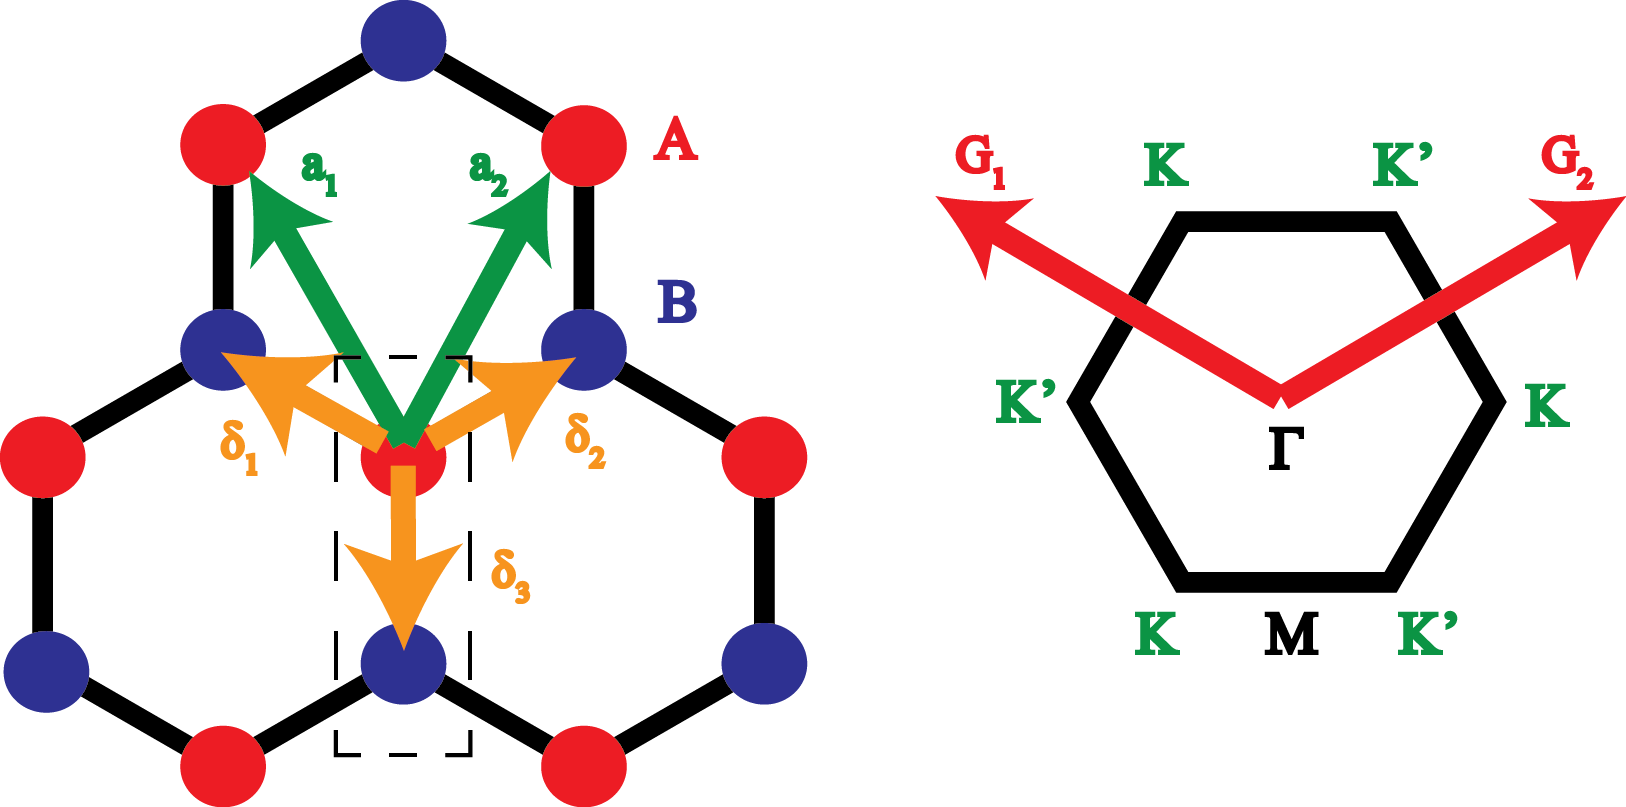
\includegraphics[width=120mm,keepaspectratio=true]{honeycomb_primitive_cell.png}
\caption{Honeycomb Lattice and Brillouin Zone}\label{Honeycomb}
\end{figure}

I now present the low energy effective theory of electrons on a honeycomb lattice.  Suppose we had a honeycomb made of two interpenetrating triangular sublattices, hereby denoted as the $A$ and $B$ sublattices (see Fig. \ref{Honeycomb}).  Each triangular sublattice can be constructed by the primitive lattice vectors
\begin{equation}
\vec{a}_1 = a \left( -\frac{\sqrt{3}}{2}, \frac{3}{2} \right), \text{ }
\vec{a}_2 = a \left( \frac{\sqrt{3}}{2}, \frac{3}{2} \right)
\end{equation}
where $a$ is the distance between a point on the $A$ sublattice (call it the origin) and its nearest neighbors on the $B$ sublattice.  The nearest neighbors are
\begin{equation}
\vec{\delta}_1 = a \left( -\frac{\sqrt{3}}{2}, \frac{1}{2} \right), \text{ }
\vec{\delta}_2 = a \left( \frac{\sqrt{3}}{2}, \frac{1}{2} \right), \text{ }
\vec{\delta}_3 = a \left( 0, -1 \right)
\end{equation}
I define a unit cell to encompass a point on $A$ and its nearest neighbor on $B$ at $\vec{\delta}_3$. \\
The reciprocal lattice vectors are
\begin{equation}
\vec{G}_1 = \frac{2 \pi}{a} \left( -\frac{1}{\sqrt{3}}, \frac{1}{3} \right), \text{ }
\vec{G}_2 = \frac{2 \pi}{a} \left( \frac{1}{\sqrt{3}}, \frac{1}{3} \right)
\end{equation}
The Brillouin Zone for a triangular lattice is a hexagon with high symmetry points $K$ and $K'$ on its corners:
\begin{equation}
\vec{K} = \frac{2 \pi}{a} \left(\frac{2}{3 \sqrt{3}}, 0 \right), \text{ }
\vec{K}' = \frac{2 \pi}{a} \left( -\frac{2}{3 \sqrt{3}}, 0 \right)
\end{equation}
Lets now consider a tight binding model with nearest neighbor hopping amplitude $t$
\begin{equation}
H= U \sum_i a_i^\dagger a_i- U \sum_j b_j^\dagger b_j - t \sum_{\langle i,j \rangle} \left( a_i^\dagger b_j + \text{h.c.} \right)
\end{equation}
where $a_i^\dagger$ and $a_i$ are the creation and annihilation operators for site $i$ on sublattice $A$ (and similarly, $b_j^\dagger$ and $b_j$ are for $B$).  $U$ is half the energy difference between an electron sitting on sublattice $B$ as opposed to $A$.  I've neglected spin and hopping further than nearest neighbor.  I've also assumed points on the $A$ and $B$ sublattice have no internal structure.
Applying this Hamiltonian to the state $|A,\vec{r} \rangle$ in which a single electron inhabits a point on sublattice $A$ in the unit cell at $\vec{r}$:
\begin{equation}
H|A,\vec{r} \rangle = U|A,\vec{r} \rangle -t \left( |B,\vec{r}+\vec{a}_1 \rangle + |B,\vec{r}+\vec{a}_2 \rangle + |B,\vec{r} \rangle \right)
\end{equation}
And similarly for $|B,\vec{r} \rangle$ in which a single electron inhabits the point on sublattice $B$ in the unit cell at $\vec{r}$:
\begin{equation}
H|B,\vec{r} \rangle = -U|B,\vec{r} \rangle -t \left( |A,\vec{r}-\vec{a}_1 \rangle + |A,\vec{r}-\vec{a}_2 \rangle + |A,\vec{r} \rangle \right)
\end{equation}
Define Bloch states
\begin{eqnarray}
|A, \vec{k} \rangle = \sum_{\vec{r}} e^{i \vec{k} \cdot \vec{r}} |A,\vec{r} \rangle \\
|B, \vec{k} \rangle = \sum_{\vec{r}} e^{i \vec{k} \cdot \vec{r}} |B,\vec{r} \rangle
\end{eqnarray}
where the sum is taken over unit cells indexed by their positions $\vec{r}$.  Applying the Hamiltonian on these Bloch states,
\begin{eqnarray}
H|A,\vec{k} \rangle &=& U|A,\vec{k} \rangle -t \sum_{\vec{r}}  e^{i \vec{k} \cdot \vec{r}} \left( |B,\vec{r}+\vec{a}_1 \rangle + |B,\vec{r}+\vec{a}_2 \rangle + |B,\vec{r} \rangle \right) \nonumber \\
 &=& U|A,\vec{k} \rangle -t \left( e^{-i \vec{k} \cdot \vec{a}_1}+e^{-i \vec{k} \cdot \vec{a}_2} +1 \right)|B, \vec{k} \rangle \\
H|B,\vec{k} \rangle &=& -U|B,\vec{k} \rangle - t \left( e^{i \vec{k} \cdot \vec{a}_1}+e^{i \vec{k} \cdot \vec{a}_2} +1 \right)|A, \vec{k} \rangle
\end{eqnarray}
Clearly, the Hamiltonian for each $\vec{k}$ subspace can be represented by the matrix
\begin{equation}
H(\vec{k})= -t \left(
\begin{array}{cc}
U & e^{-i \vec{k} \cdot \vec{a}_1}+e^{-i \vec{k} \cdot \vec{a}_2} +1  \\
e^{i \vec{k} \cdot \vec{a}_1}+e^{i \vec{k} \cdot \vec{a}_2} +1 & -U
\end{array}
\right)
\end{equation}
We can rewrite the Hamiltonian in terms of the Pauli matrices $\sigma_x$, $\sigma_y$, and $\sigma_z$ if I define
\begin{eqnarray}
X(\vec{k}) &=& -t \left[ 1+ \cos \left( \frac{\sqrt{3}}{2}k_x a - \frac{3}{2}k_y a \right) + \cos \left( -\frac{\sqrt{3}}{2}k_x a - \frac{3}{2}k_y a \right) \right] \\
Y(\vec{k}) &=& t \left[ \sin \left( \frac{\sqrt{3}}{2}k_x a - \frac{3}{2}k_y a \right) + \sin \left( -\frac{\sqrt{3}}{2}k_x a - \frac{3}{2}k_y a \right) \right]
\end{eqnarray}
so that $H(\vec{k})=X(\vec{k}) \sigma_x + Y(\vec{k}) \sigma_y+U \sigma_z$.  At this point, we can calculate the energy $E(\vec{k})=\sqrt{X(\vec{k})^2+Y(\vec{k})^2+U^2}$ for all $\vec{k}$ in the Brillouin Zone.  However, for reasons that will become clear, lets expand $X(\vec{k})$ and $Y(\vec{k})$ around the $K$ point (i.e., let $\vec{k}=\vec{K}+\vec{q}$):
\begin{eqnarray}
X(\vec{k}) &=& -t \left[ 1+ \cos \left(\frac{2 \pi}{3} + \frac{\sqrt{3}}{2}q_x a - \frac{3}{2}q_y a \right) + \cos \left( -\frac{2 \pi}{3} - \frac{\sqrt{3}}{2}q_x a - \frac{3}{2}q_y a \right) \right] \nonumber \\
&\approx& -t \left[ -\frac{\sqrt{3}}{2} \left( \frac{\sqrt{3}}{2}q_x a - \frac{3}{2}q_y a \right) + \frac{\sqrt{3}}{2} \left( -\frac{\sqrt{3}}{2}q_x a - \frac{3}{2}q_y a \right) \right] \approx \frac{3at}{2} q_x \\
Y(\vec{k}) &=& t \left[ \sin \left(\frac{2 \pi}{3} + \frac{\sqrt{3}}{2}q_x a - \frac{3}{2}q_y a \right) + \sin \left( -\frac{2 \pi}{3} - \frac{\sqrt{3}}{2}q_x a - \frac{3}{2}q_y a \right) \right] \nonumber \\
&\approx& t \left[ -\frac{1}{2} \left( \frac{\sqrt{3}}{2}q_x a - \frac{3}{2}q_y a \right) - \frac{1}{2} \left( -\frac{\sqrt{3}}{2}q_x a - \frac{3}{2}q_y a \right) \right] \approx \frac{3at}{2} q_y
\end{eqnarray}
Thus,
\begin{equation}
H(\vec{q})=\hbar v_F \left( q_x \sigma_x + q_y \sigma_y \right) + U \sigma_z
\end{equation}
where $v_F=\frac{3at}{2\hbar}$.  This is a form of the two-dimensional Dirac Equation with mass $U$ and the speed of light replaced by $v_F$.  A similar expansion can be performed near $K'$. \\
Graphene is similar to this tight binding model in that the electrons in graphene hop between the out-of-plane p orbitals.  For graphene, there is no energy difference between $A$ and $B$, so $U=0$:
\begin{equation}
H(\vec{p})= v_F \vec{p} \cdot \vec{\sigma}
\end{equation}
where $\vec{p}=\hbar \vec{q}$ and $\vec{\sigma}=(\sigma_x,\sigma_y)$.  This leads to the energy-momentum dispersion $E=\pm \hbar v_F q$.  Note that there are two symmetric conical bands that meet at $E=0$, the so-called ``Dirac Point."  I will use terminology such as ``electron-like band," ``top band," or $\pi^*$ band to describe the positive energy states.  Likewise, I will refer to the negative energy states as being in the ``hole-like band," ``bottom band," or $\pi$ band. \\
Lets define $\phi$ such that $\vec{q}=(q_x,q_y)=q(\cos(\phi),\sin(\phi))$.  Then the graphene Hamiltonian can be rewritten as
\begin{equation}
H(\vec{q})= \hbar v_F q \left(
\begin{array}{cc}
0 & e^{-i \phi}  \\
e^{i \phi} & 0
\end{array}
\right)
\end{equation}
which has eigenvectors
\begin{equation}
\Psi_{\vec{K}, \pi^*} (\vec{q} )=\frac{1}{\sqrt{2}} \begin{pmatrix}
e^{-i \phi/2} \\ e^{i \phi/2}
\end{pmatrix}, \text{ }
\Psi_{\vec{K}, \pi} (\vec{q} )=\frac{1}{\sqrt{2}} \begin{pmatrix}
e^{-i \phi/2} \\ -
e^{i \phi/2}
\end{pmatrix}
\end{equation}
Note the similarity to a spin pointing in the $\phi$ direction.  For this reason, the sublattice degree of freedom is referred to as ``pseudospin."  However, unlike the real spin for a massive particle, pseudospin is locked parallel or antiparallel to $\vec{q}$.  Thus, while there is spin degeneracy, there is no pseudospin degeneracy.  On the other hand, graphene does have a ``valley" degeneracy arising from the symmetry between $K$ and $K'$.

\end{document}